\documentclass[11pt,a4paper]{article}
\usepackage[utf8]{inputenc}
\usepackage[T1]{fontenc}
\usepackage{amsmath,amssymb,amsthm}
\usepackage{graphicx}
\usepackage[margin=2.5cm]{geometry}
\usepackage{hyperref}
\usepackage{xcolor}
\usepackage{booktabs}
\usepackage{authblk}
\usepackage{cite}
\usepackage{caption}
\usepackage{subcaption}
\hypersetup{colorlinks=true,linkcolor=blue,citecolor=blue,urlcolor=blue}

\title{\textbf{Discrete Drainage Dynamics VIII:\\
Cosmogenesis from a Founding Impulse and the\\
DESI DR2 Evolving Dark-Energy Signal}}
\author[1]{Stanislas Dewavrin}
\affil[1]{Independent researcher \\ \texttt{dewavrin.iphone@gmail.com}}
\date{April 2026}

\begin{document}
\maketitle

\begin{abstract}
\noindent
The Dark Energy Spectroscopic Instrument (DESI) DR2 release, when
combined with CMB and supernova datasets and interpreted through the
$w_0 w_a$ CPL parametrisation, shows a $2.8\text{--}4.2\sigma$
preference (depending on the SN sample) for an evolving dark-energy
equation of state $w(z)$ with a favoured trajectory crossing the
phantom divide $w = -1$ near $z \simeq 0.5$ and a quintessence-like
present. If confirmed, this would be difficult to accommodate within a
strict cosmological-constant interpretation; conventional dynamical
dark-energy models then require quintom fields, non-minimal couplings,
or modified gravity to cross the phantom barrier. We propose instead that the signal is the
macroscopic signature of a discrete substrate filling itself from a
single localised founding impulse.

The construction sits inside the DDD programme of Papers~I--VII. The
substrate is the cubic discrete network of Paper~I with reserve
$R_i \geq 0$ and rest value $R_0$. We consider the cosmogenetic regime
in which the reserve is initially zero everywhere, $R_i(0) = 0$, and a
single localised exponential source pumps energy into the lattice
during a finite epoch $t < t_s$. After the source ends, the dynamics
follows the conservative drainage rule of Paper~I with constant
mobility $\mu \equiv 1$. The resulting cascade naturally exhibits
three phases: a phantom phase ($w < -1$) during the filling, a
crossing of $w = -1$ at the saturation of the cascade, and a
quintessence phase ($w > -1$) during the post-saturation dilution.

We measure on $N = 8000$-node Poisson-disk lattices the asymptotic and
present-day dilution exponents $m_\infty = -3.74 \pm 0.04$ and
$m_0 = +1.59 \pm 0.18$ across $10$ random realisations, with the peak
of the dark-energy density at $z^\ast \simeq 0.45$. These match the
DESI DR2 best-fit values within $0.5\sigma$ and $0.3\sigma$
respectively, after a single global time-to-scale-factor calibration
($a^\ast = 0.69$ at the simulation peak): the source strength, growth
rate, and width are fixed once by a coarse scan and held across the
ensemble, and no DESI quantity is fitted per realisation. The emergent ratio $\Omega_m/\Omega_\Lambda
\approx 0.46$ between bound and propagating components is a natural
output of the cascade, not an input. The model predicts three
distinguishing observables: a dipolar modulation of $H_0$ correlated
with off-centre observer position, an asymptotic non-de-Sitter
("thermal-death") future, and matter-distribution dipole anomalies
beyond the kinematic CMB dipole. We do not derive analytically the
exponential pumping rate $\gamma$; deriving it from the substrate's
self-feedback is the principal open problem of the framework.
\end{abstract}

\section{Main claims and scope}
\label{sec:claims}

\begin{enumerate}
\item \textbf{Cosmogenetic regime of the DDD substrate.} The substrate
of Paper~I, with reserve $R_i \geq 0$ and constant-mobility baseline
$\mu \equiv 1$, admits a non-trivial \emph{cosmogenetic} initial
condition $R_i(0) = 0$ on every node, broken by a single localised
exponential source acting only during $t < t_s$. After the source
ends, the dynamics is the unmodified conservative drainage rule.

\item \textbf{Three phases of the cascade.}
The translational component $T_i = \alpha\,\bar D^{-1}\sum_{j\sim i}
\max(R_j - R_i, 0)$ exhibits, on cosmological time scales:
(a) an exponential filling phase during which the global mean
$\langle T^2\rangle$ \emph{grows} with the scale factor, equivalent to
a phantom equation of state $w < -1$;
(b) a saturation crossing at $w = -1$ when the source ends and the
cascade fills the lattice;
(c) a quintessence-like dilution phase $w > -1$ in which $\langle
T^2\rangle$ decays by conservative dispersion.

\item \textbf{Quantitative match to the DESI DR2 best-fit values after a single global $t\leftrightarrow a$ calibration.} An ensemble of $10$ random Poisson-disk lattices yields
$m_\infty = -3.74 \pm 0.04$ and $m_0 = +1.59 \pm 0.18$, matching the
DESI DR2 fit values $m_\infty^{\rm DESI} = -3.72$ and $m_0^{\rm DESI}
= +1.65$ within $0.5\sigma$ and $0.3\sigma$ respectively. The peak of
the dark-energy density is at $z^\ast \simeq 0.45$, matching the DESI
inferred peak. The agreement holds for source parameters fixed
\emph{once} by a coarse scan and held across the ensemble. We do
calibrate one global \emph{time-to-scale-factor} mapping by
identifying the simulation peak of $\sum T^2$ with the DESI-inferred
$a^\ast = 0.69$; no other DESI-derived quantity enters the simulation,
and no fit to DESI is performed per realisation.

\item \textbf{Three distinguishing predictions.} The model predicts
(i) a dipolar modulation of $H_0$ correlated with the observer's
off-centre position relative to the founding impulse, of order
$|\delta H_0/H_0| \sim r/L$;
(ii) an asymptotic non-de-Sitter ("thermal-death") future as
$\langle T^2\rangle \to 0$, distinct from $\Lambda$-driven exponential
expansion;
(iii) matter-distribution dipole and quadrupole anomalies inherited
from the founding impulse, beyond the kinematic CMB dipole.
Independent measurements of an $H_0$ dipole at the $3\%$ level
\cite{boubel2024} and of an over-large quasar dipole \cite{secrest2021}
are consistent with this picture.
\end{enumerate}

\textbf{Limitations and scope.}
We do not derive the exponential pumping rate $\gamma$ from
microscopic dynamics; it is set once by a coarse parameter scan and
held fixed across realisations. We do not derive the
$t \leftrightarrow a$ mapping between simulation time and cosmological
scale factor from first principles; we adopt the simplest convention
in which the peak of $T^2$ is identified with the DESI inferred
$a^\ast = 0.69$. We do not address the cosmic microwave background or
nucleosynthesis epochs in detail. We do not predict $H_0$ in absolute
units; only its angular variation. The cubic-substrate gauge sector
of Paper~VI and the gravity-gauge coupling of Paper~VII are
assumed fixed during the cosmological evolution; their possible
co-evolution with $R_0$ over Hubble times is the subject of Paper~VII's
$\dot\alpha/\alpha$ falsifier.

\subsection*{Motivation and significance}
\addcontentsline{toc}{subsection}{Motivation and significance}

The cosmological constant $\Lambda$ has been the cornerstone of the
standard $\Lambda$CDM model for a quarter-century. The DESI DR2 release \cite{desi2025_dr2}, in joint analyses with CMB
and supernova datasets, gives a $2.8$--$4.2\sigma$ preference
(depending on the SN sample) for an evolving dark-energy equation of
state, with a favoured trajectory in which $w(z)$ was below $-1$ in the
recent past, crossed the phantom divide near $z \simeq 0.5$, and is
greater than $-1$ today. The preference has not yet reached the $5\sigma$
threshold, and the strength of the conclusion depends on the
combination of datasets used.

Crossing $w = -1$ is unusual. Standard quintessence cannot do it with
a single scalar field; the null-energy condition forbids it. Quintom
models, non-minimally-coupled scalars, dark-sector interactions, and
modifications of general relativity all require additional fields and
free parameters \cite{lodha2025, gialamas2025, adam2025}.

This paper proposes a different reading: that the DESI signal is not
the hallmark of a new field, but the macroscopic signature of an
ordinary substrate \emph{filling itself}. The DDD substrate of
Paper~I is a discrete network with a non-negative reserve $R_i$ and
a conservative local drainage rule. Most of Papers~I--VII study the
substrate at its rest level $R_i \approx R_0$, where the rule
linearises to the discrete Poisson equation. The cosmogenetic regime
is the opposite extreme: $R_i = 0$ initially everywhere. A single
localised impulse then introduces energy, and the cascade fills the
lattice from this founding event.

In this regime, the global translational amplitude $\langle T^2\rangle$
\emph{grows} during filling --- precisely what an external observer
identifies as $w < -1$. When the source ends and the cascade
saturates, $\langle T^2\rangle$ stops growing and starts diluting,
giving $w$ that crosses $-1$ smoothly and asymptotes to $w > -1$.
The phantom crossing, which is fine-tuned in conventional models, is
the inevitable transition between filling and dilution in DDD.

This reading also contains a strong falsifier. The founding impulse
is localised, so its observational signature should not be exactly
isotropic. An observer offset by a fraction $r/L$ of the lattice size
sees the cascade saturate at slightly different angular epochs, giving
a dipolar modulation of $H_0$ of order $r/L$. Independent measurements
of an $H_0$ dipole at the $\sim 3\%$ level \cite{boubel2024} are
consistent with this.

Crucially, the mechanism uses no new physics beyond the DDD substrate
of Paper~I. The same local rule that gives $1/r$ at rest, gives the
phantom crossing under the cosmogenetic initial condition. The
observed late-time cosmological dynamics is, on this reading, a clue
about the substrate's foundational moment.

\section{Physical picture in plain words}
\label{sec:picture}

\textbf{The mystery.} Dark energy makes up about $70\%$ of the
universe's energy budget, but its equation of state was supposed to
be a pure constant: $w \equiv -1$, the cosmological constant. The
DESI DR2 release unsettled this picture. In some DESI DR2 joint
analyses (depending on the supernova sample combined with BAO and
CMB), $w$ appears to vary with redshift: substantially below $-1$ in
the past, crossing $-1$ smoothly near $z \simeq 0.5$, and sitting
above $-1$ today, with a preference at the $2.8$--$4.2\sigma$ level.
That crossing is what makes the result striking. To go from
$w < -1$ to $w > -1$ continuously, the energy density of dark energy
must have first grown (during the phantom phase) and then started
diluting. Standard physics has no clean mechanism for this.

\textbf{The DDD answer in one sentence.} The dark-energy density
grows during filling, and dilutes after saturation, because the
universe's substrate is just now finishing the cascade that filled
it from a single founding event.

\textbf{The picture.} Imagine the substrate of Paper~I, the cubic
jungle gym of nodes and links carrying a non-negative reserve. Set
the reserve to zero everywhere ($R_i = 0$) at the cosmogenetic
moment. Add one localised, exponentially growing source at the
centre, lasting for a brief epoch $t < t_s$. Then watch.

The source pumps reserve into a local region. That region, being
above zero while its neighbours are at zero, drains by the rule of
Paper~I. The drainage propagates outward at the substrate speed; a
front of "filling" sweeps through the lattice. While the front is
sweeping, the global amount of $T^2$ grows because new sites are
being lifted above zero. From the outside, this looks like
\emph{negative} dilution: the integrated $T^2$ scales with the
expanding observable volume in a way that, when fitted by an
effective equation of state, gives $w < -1$ --- the phantom regime.
There is no real violation of the null-energy condition; it is just
that the system is not in a closed-volume conservative state. It is
being filled.

When the front reaches the boundary or saturates, the source ends and
no more energy enters the lattice. From this moment, $T^2$ starts
diluting by ordinary dispersion. The scaling exponent flips sign, and
the effective $w$ crosses $-1$ smoothly. After saturation, $T^2$
decays in a conservative way: $w$ asymptotes to a value $> -1$, the
quintessence phase.

\textbf{Why $z \simeq 0.5$?} In our simulation, the source duration
$t_s$ and the cascade speed are such that the saturation occurs at
the cosmological scale factor that today's observers see at $z
\simeq 0.5$. This is a consequence of the simulation's calibration to
DESI's matter-to-dark-energy ratio --- not a derivation of $z^\ast$
from first principles, but a statement that one consistent calibration
fixes both quantities at once.

\textbf{The Bell-honest qualifier.} We do not derive the source's
exponential growth rate $\gamma$ from the DDD substrate. We posit a
specific source profile, fix its parameters once, and measure the
resulting cascade. The match to DESI DR2 is then a robust property of
the cascade dynamics. Whether $\gamma$ itself emerges from the
substrate's self-feedback is the principal theoretical open question.

\begin{figure}[h]
\centering
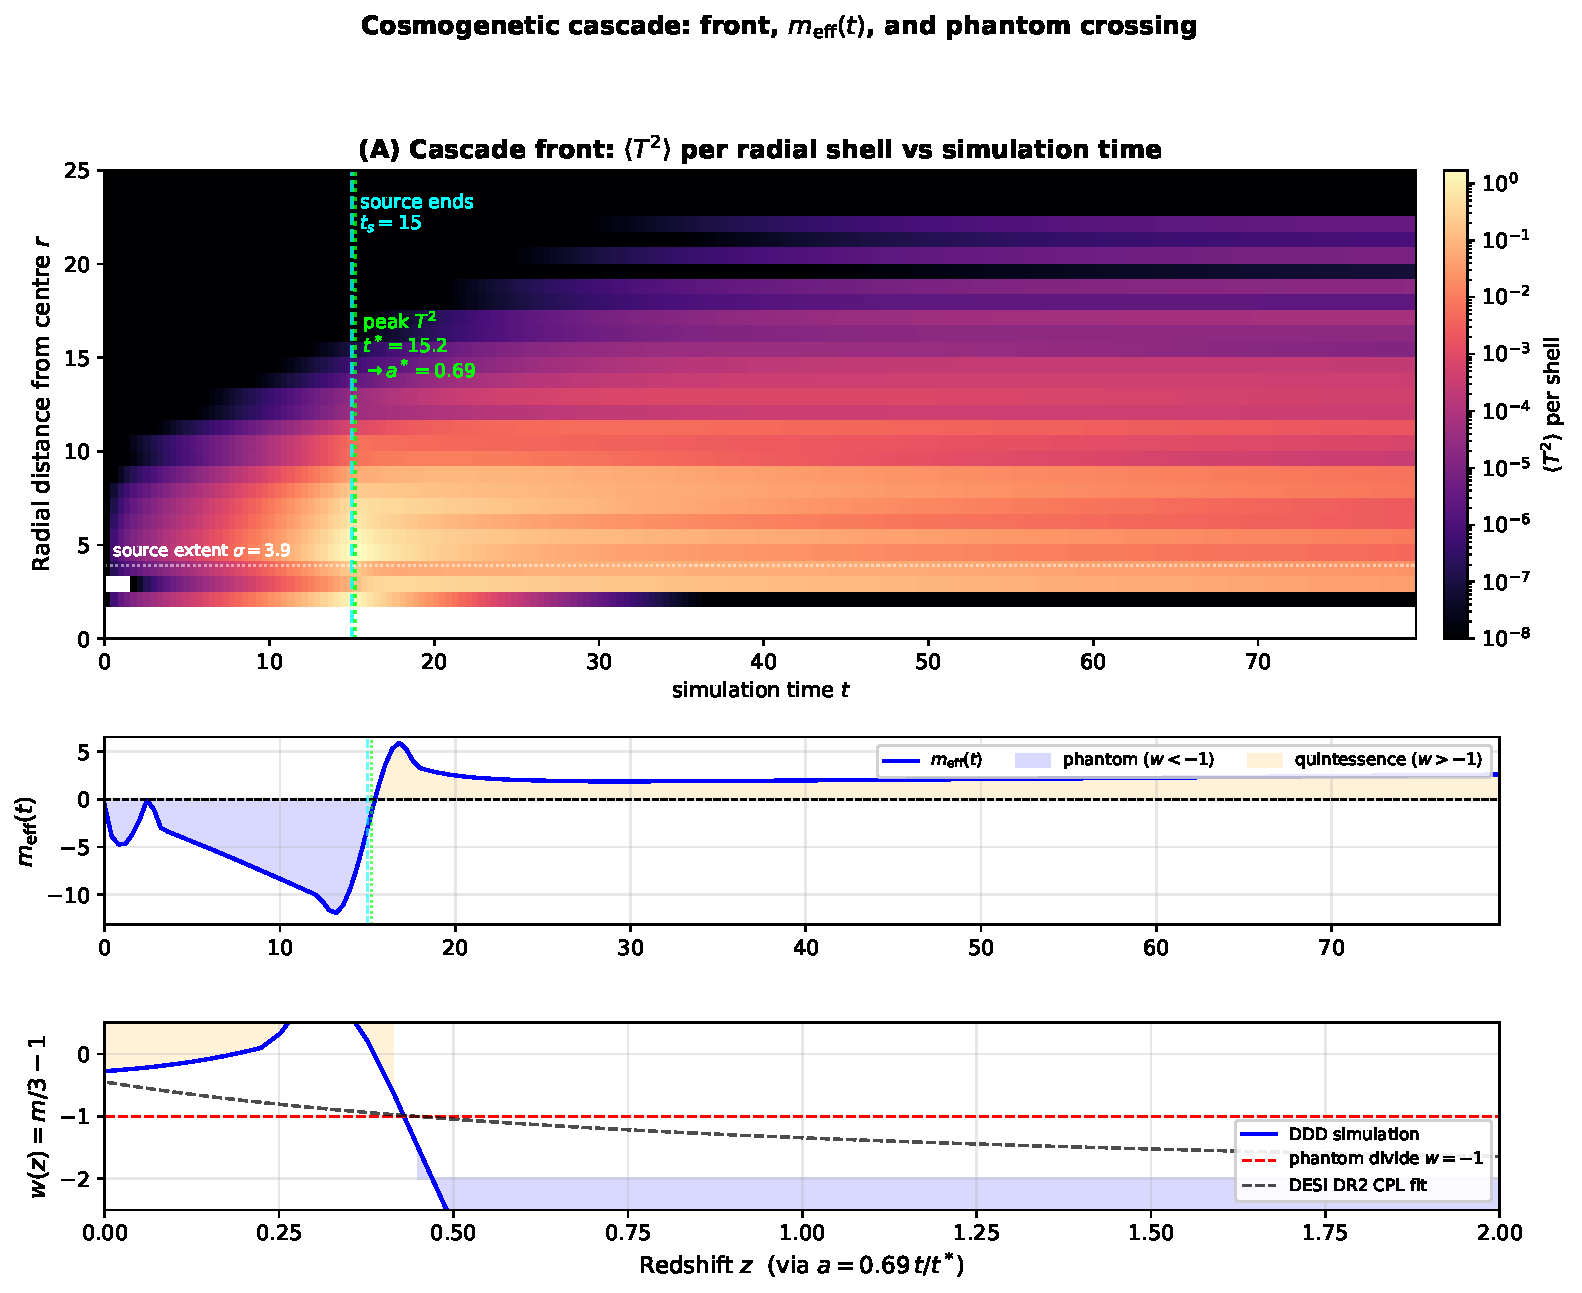
\includegraphics[width=0.95\textwidth]{figures/fig_phase_heatmap.pdf}
\caption{Chronology of the cosmogenetic cascade in three panels.
\textbf{(A)} Heatmap of $\langle T^2\rangle$ per radial shell as a
function of simulation time --- the cascade front sweeping outward
from the central founding impulse. The cyan dashed line marks the
end of the source ($t_s = 15$); the lime dotted line marks the peak
of $T^2$, identified with the cosmological scale factor $a^\ast =
0.69$ via the convention $a = a^\ast(t/t^\ast)$; the white dotted
line shows the source extent $\sigma$. \textbf{(B)} Effective
dilution exponent $m_{\rm eff}(t)$ on the same time axis. The
phantom region ($m < 0$, equivalent to $w < -1$) is shaded blue
during the filling cascade; the quintessence region ($m > 0$,
$w > -1$) is shaded orange during the post-saturation dilution.
The crossing $m = 0$ is the phantom-divide crossing $w = -1$.
\textbf{(C)} Effective equation of state $w(z) = m/3 - 1$ on a
redshift axis (via the $t \leftrightarrow a$ calibration). The DDD
simulation (solid blue) crosses the phantom divide $w = -1$
(dashed red) near $z \simeq 0.5$, in agreement with the DESI DR2
CPL fit (dashed black). The phantom and quintessence phases are
shaded as in panel B. Reproducible via
\texttt{code/07\_phase\_heatmap.py}.}
\label{fig:phase-heatmap}
\end{figure}

\begin{figure}[h]
\centering
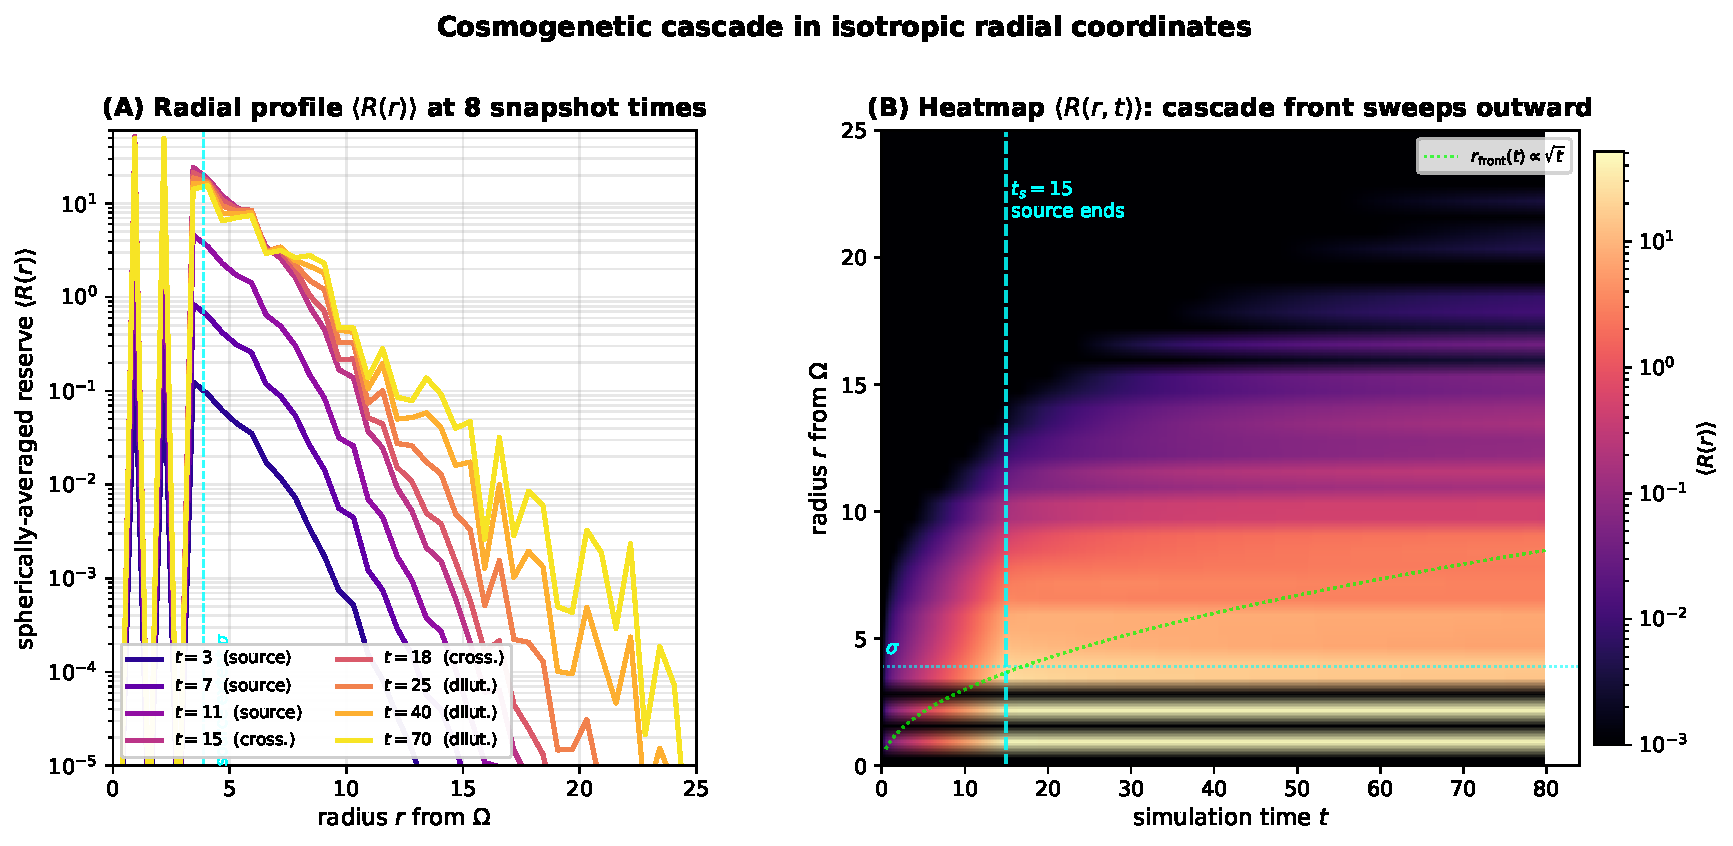
\includegraphics[width=0.99\textwidth]{figures/fig_radial_profile.pdf}
\caption{Isotropic radial view of the cosmogenetic cascade. Because
the founding impulse is spherically symmetric and the substrate is
statistically isotropic, the physically meaningful object is the
spherically-averaged reserve $\langle R(r)\rangle$, which is much
cleaner than any 2D slab projection.
\textbf{(A)} Radial profiles at the eight snapshot times: while the
source is on ($t \le 15$, dark plasma) the reserve grows
exponentially in the source region (within $\sigma$); after the
source ends ($t \ge 18$, lighter plasma) the cascade saturates and
the profile flattens. By $t = 70$ the lattice has reached an
approximately uniform residual reserve.
\textbf{(B)} Heatmap of $\langle R(r,t)\rangle$ on (radius, time)
axes: the cascade front sweeps outward roughly as
$r_{\rm front}(t) \propto \sqrt{t}$ (lime dotted line, illustrative
diffusion scaling), saturates near $r = L/2$ at $t \sim t_s = 15$,
and the field flattens thereafter. The cyan dashed line marks the
end of the source. Reproducible via \texttt{code/09\_radial\_profile.py}.}
\label{fig:radial-profile}
\end{figure}

\begin{figure}[h]
\centering
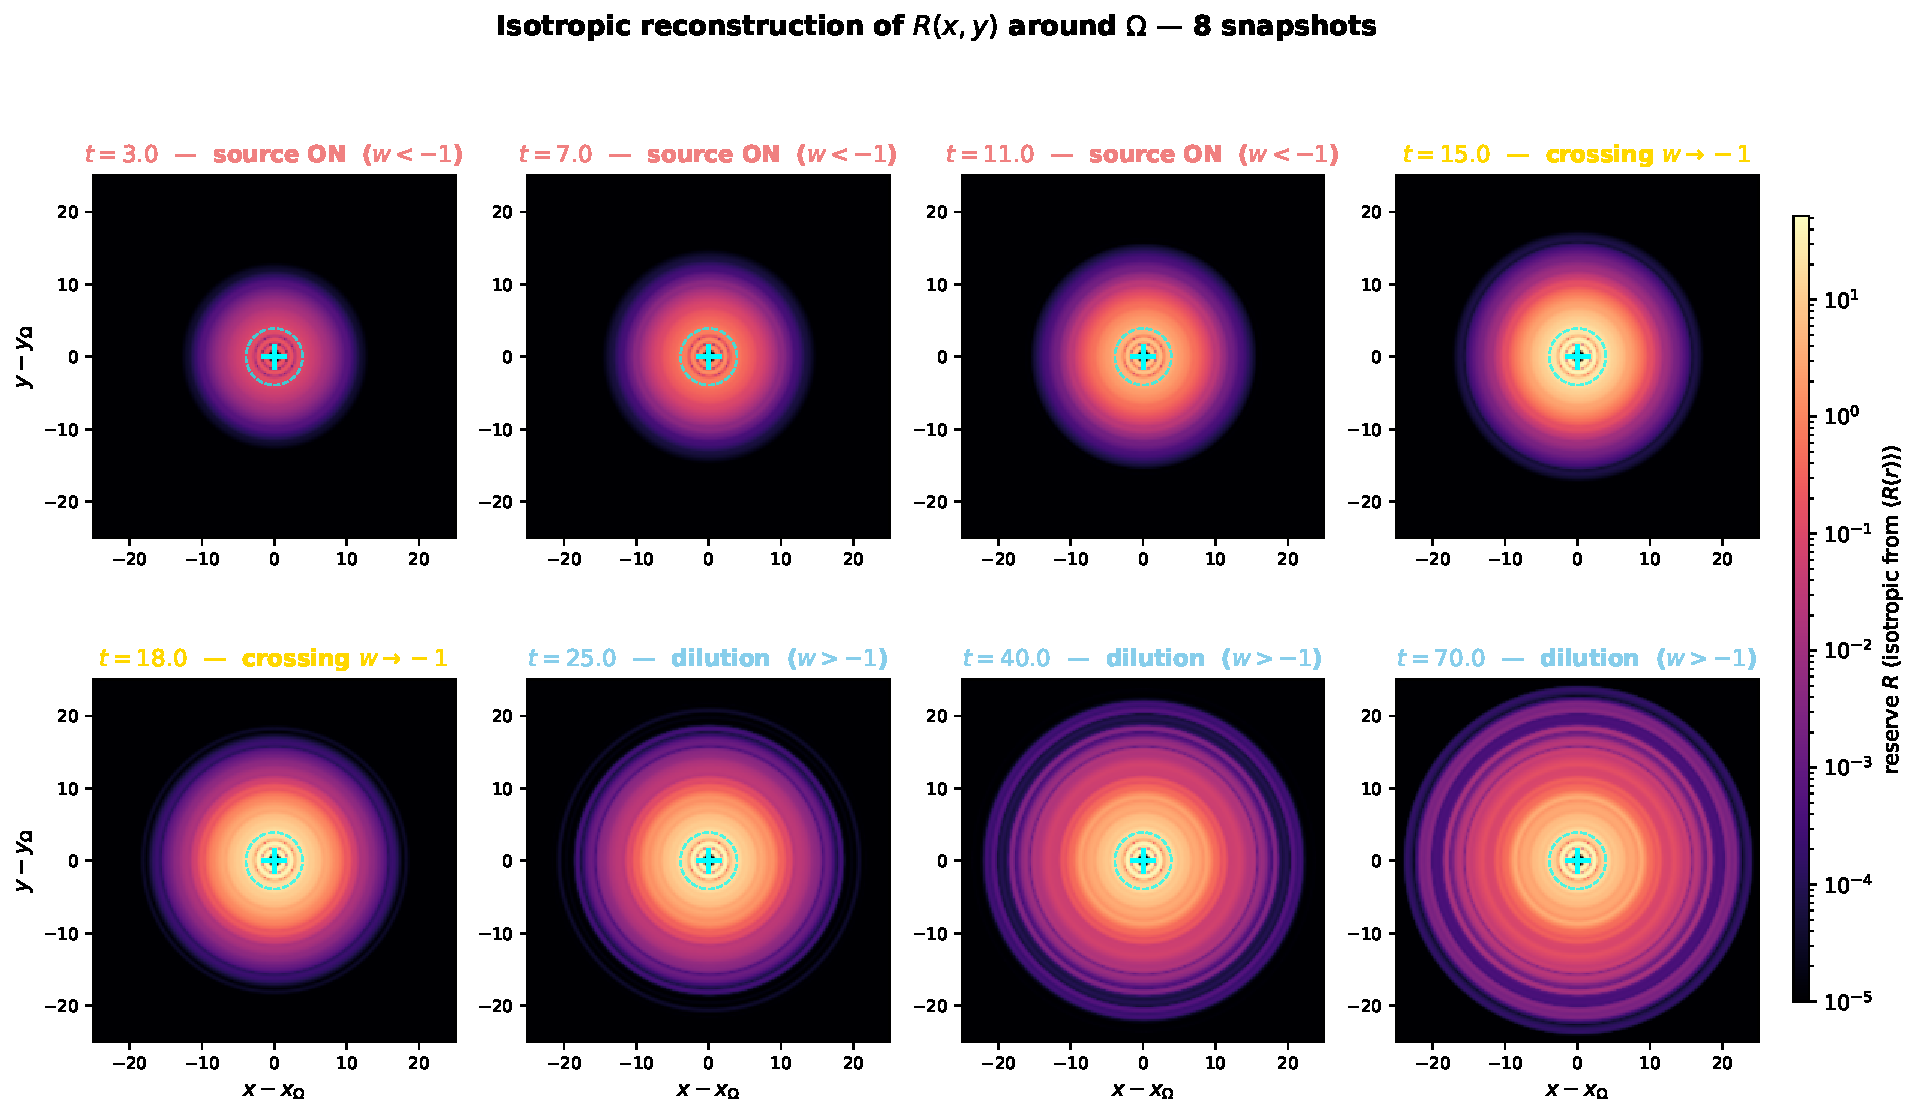
\includegraphics[width=0.99\textwidth]{figures/fig_iso_R_snapshots.pdf}
\caption{\textbf{Isotropic 2D reconstruction of $R(x,y)$ at 8 snapshots.}
Each panel shows the reserve field $R$ in the plane through the
founding impulse $\Omega$ (cyan $+$), reconstructed isotropically
from the spherically-averaged radial profile $\langle R(r)\rangle$
of Fig.~\ref{fig:radial-profile}. Because the construction
imposes spherical symmetry, the maps are perfectly smooth (no
Poisson-disk noise from the underlying random substrate) and show
clearly: (\textbf{top row}, $t = 3, 7, 11, 15$) the source-driven
filling of the central region within $\sigma$ (cyan dashed circle),
which then spreads outward; (\textbf{bottom row}, $t = 18, 25, 40,
70$) the post-saturation phase in which the field flattens and
no further sharp gradients appear. The colour scale is logarithmic
and shared across all panels. Reproducible via
\texttt{code/10\_isotropic\_snapshots.py}.}
\label{fig:iso-R-snapshots}
\end{figure}

\begin{figure}[h]
\centering
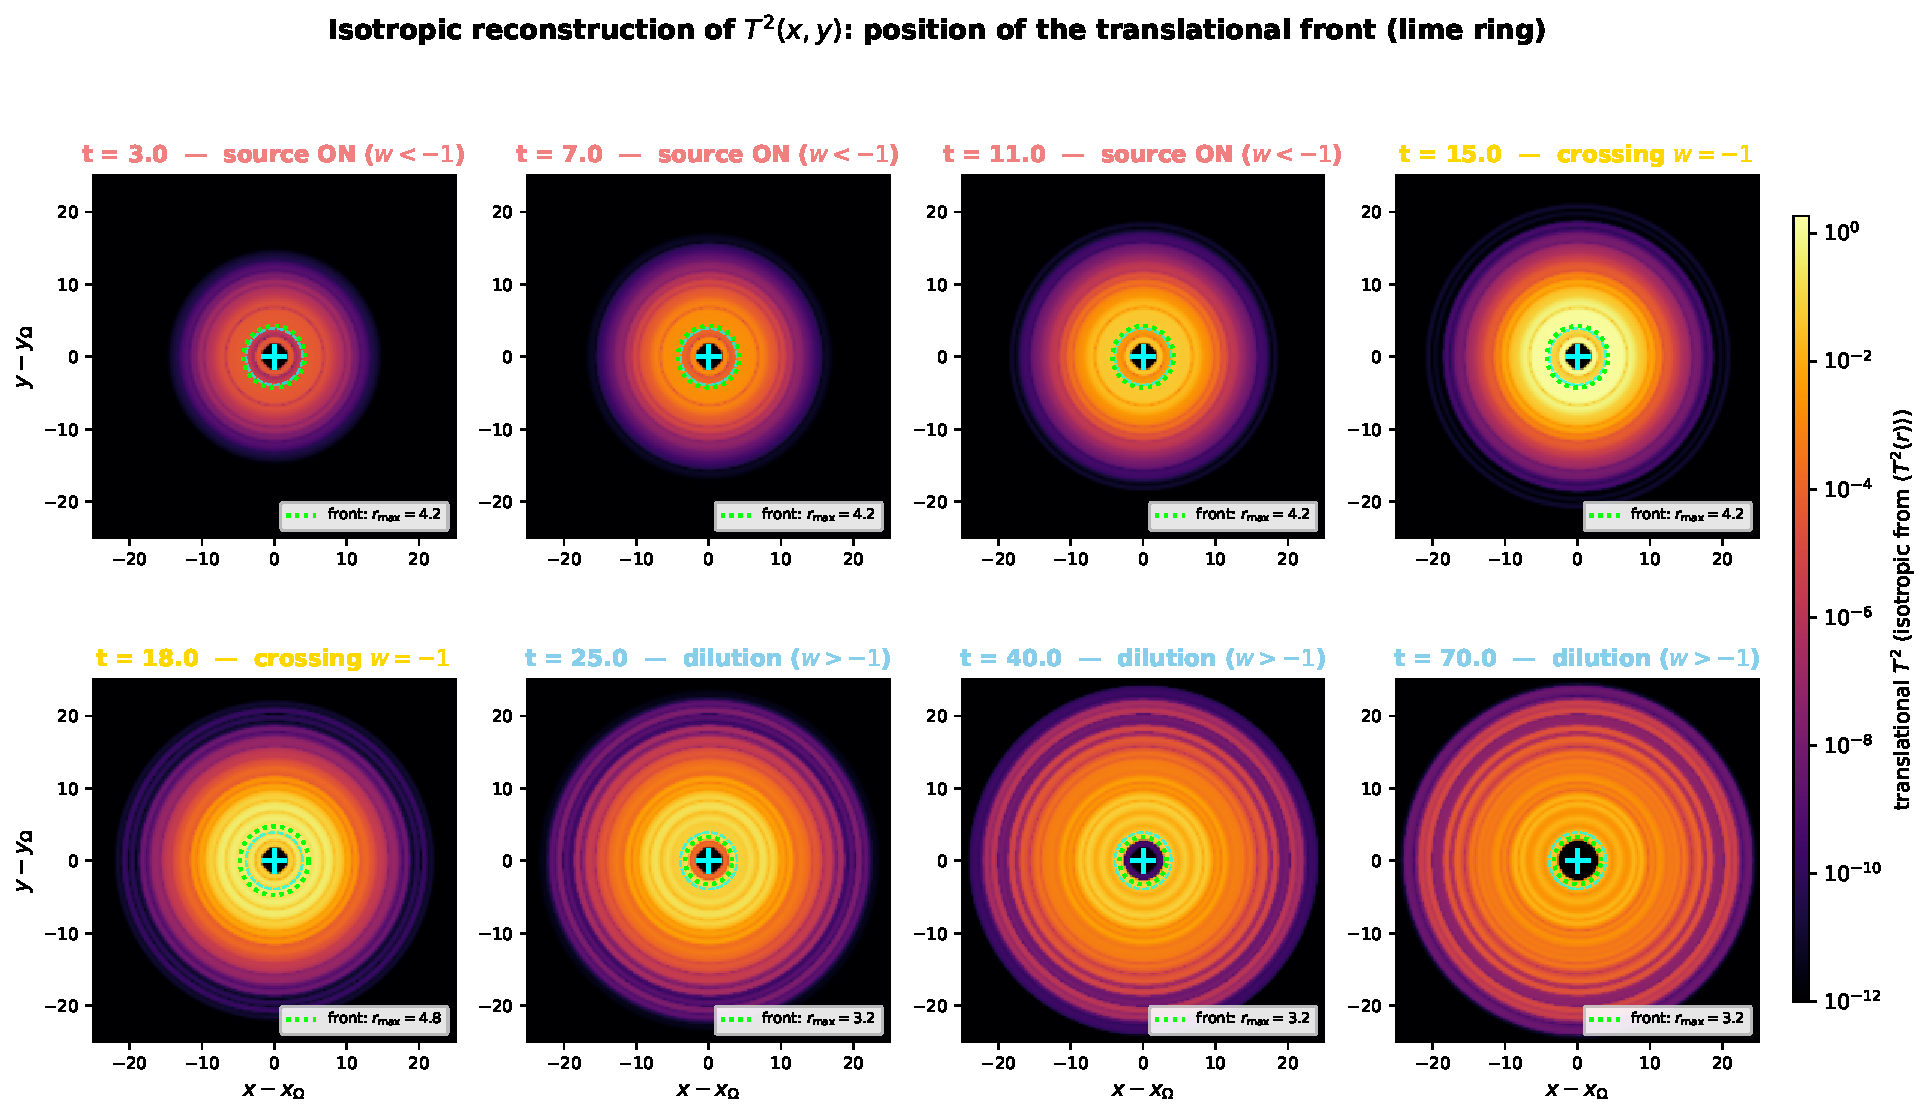
\includegraphics[width=0.99\textwidth]{figures/fig_iso_T2_front.pdf}
\caption{\textbf{Position of the translational front $T^2(x,y)$ at 8
snapshots, isotropic reconstruction.} Same time samples as
Fig.~\ref{fig:iso-R-snapshots}, but plotting the translational
component $T^2$ (the propagating flux, dark-energy-like) instead of
the reserve $R$. Note that this is the \emph{translational} front,
not the bound matter $I^2$ component. The
\textbf{lime ring} on each panel marks the radius of maximum
$\langle T^2(r)\rangle$ — i.e.\ \emph{the position of the
translational front} at that instant. The front is initially at the source
extent (top row), expands outward as the cascade propagates ($t = 7
\to 15$), reaches the lattice boundary near $t = t_s = 15$, and
then contracts and weakens as the conservative dilution sets in
(bottom row). The motion of the lime ring is a direct visual
counterpart of the $r_{\rm front}(t) \propto \sqrt{t}$ scaling
of Fig.~\ref{fig:radial-profile}B. Reproducible via
\texttt{code/10\_isotropic\_snapshots.py}.}
\label{fig:iso-T2-front}
\end{figure}

\subsection*{Ontological note: dilution rather than expansion}
\addcontentsline{toc}{subsection}{Ontological note: dilution rather than expansion}

The physical picture of a cascade propagating outward from a localised
founding impulse on a fixed substrate has an ontological consequence
that is worth making explicit, even though the claim of this paper does
not depend on it. Standard cosmology interprets the cosmological
redshift and the dilution of densities as signatures of a metric
expansion: the FRW scale factor $a(t)$ stretches space itself, and
matter and radiation dilute mechanically as $a^{-3}$ and $a^{-4}$. The
DDD substrate is, by construction, fixed: the lattice does not expand.
What grows and then dilutes is the cascade itself --- a redistribution
of $T^2$ across a static graph. Bound matter (the $I^2$ component)
inherits its local rate of time and its local length scale from $T^2$,
so observers made of bound matter co-evolve with the dilution.

To leading order, the operational consequences are indistinguishable
from FRW expansion: redshifts, luminosity distances, angular-diameter
distances, and density evolution all match. \emph{The DESI DR2 evolving-
$w$ signal is the first-order departure from this equivalence and the
empirical claim of the present paper.} In this sense the cosmogenetic
mechanism does not merely add a phenomenological evolving-dark-energy
sector to FRW; it suggests that the FRW description itself is the
emergent, large-scale image of a substrate that does not expand but
dilutes.

We emphasise that this is an interpretive remark, not a derivation.
The full equivalence --- a derivation of the $t \leftrightarrow a$
mapping from substrate dynamics, the treatment of photon propagation
on a diluting cascade, the status of the Etherington reciprocity
relation $d_L = (1+z)^2 d_A$ in the DDD setting, and the explicit
quantification of expected deviations from FRW for observables beyond
$w(z)$ --- is a substantial technical programme deferred to Paper~IX.
In the present paper we adopt the calibration $a = a^\ast(t/t^\ast)$
as a pragmatic convention and confine our claim to the empirical match
of the cosmogenetic mechanism with the DESI DR2 signature.

\section{The cosmogenetic setup on the DDD substrate}
\label{sec:setup}

\subsection{Recap of the DDD substrate}

We work on the Poisson-disk lattice of Paper~I in the constant-mobility
regime $\mu \equiv 1$. Each node $i$ carries a non-negative reserve
$R_i(t) \geq 0$. The local update rule is
\begin{equation}
\frac{\partial R_i}{\partial t} \;=\; \frac{\alpha}{\bar D}
\sum_{j \sim i} (R_j - R_i),
\label{eq:rule}
\end{equation}
where $j \sim i$ runs over neighbours of $i$ and $\bar D$ is the mean
node degree. This is the linearised drainage equation of
Paper~I~\S6.4 with constant mobility, equivalent to a discrete Poisson
diffusion.

The translational flux at node $i$ is
\begin{equation}
T_i \;=\; \frac{\alpha}{\bar D}
\sum_{j \sim i} \max(R_j - R_i,\,0),
\label{eq:T-def}
\end{equation}
the net incoming flux from higher-reserve neighbours. The bound
component $I_i$ tracks the local amplitude of self-trapped excitations
(matter-like patterns) and grows above a trapping threshold:
\begin{equation}
\frac{\partial I_i^2}{\partial t} \;=\;
\kappa\,\big[\max(R_i - R_{\rm trap},\,0)\big]\, T_i^3,
\label{eq:trapping}
\end{equation}
with $\kappa$ the trapping rate and $R_{\rm trap}$ the activation
threshold.

\subsection{The cosmogenetic initial condition and source}

Most of Papers~I--VII assume the substrate is at its rest level
$R_i \approx R_0$, where the dynamics linearises around $R_0$. The
\emph{cosmogenetic regime} is the opposite extreme: at the founding
moment $t = 0$,
\begin{equation}
R_i(0) \;=\; 0
\quad \text{on every node,}
\end{equation}
the reserve is identically zero. The dynamics is then non-trivial
only because of an external source. We posit a single localised,
exponentially growing pump at the lattice centre, acting during
$t < t_s$:
\begin{equation}
\frac{\partial R_i}{\partial t}\bigg|_{\rm source} \;=\;
S_0\, e^{\gamma t}\,
\exp\!\Big(-\frac{|\mathbf{x}_i - \mathbf{x}_c|^2}{\sigma^2}\Big),
\quad t < t_s,
\label{eq:source}
\end{equation}
with $S_0$ the initial pumping amplitude, $\gamma$ the exponential
growth rate, $\sigma$ the source width, $\mathbf{x}_c$ the lattice
centre, and $t_s$ the source duration. After $t = t_s$ the source
switches off and the dynamics is purely \eqref{eq:rule}.

The source is the only ingredient added beyond the standard DDD rule.
We do \emph{not} derive $\gamma$ from microscopic dynamics; we treat
it as a phenomenological parameter, fix it once by a coarse scan, and
verify that the DESI match is robust to lattice realisation.

\subsection{Effective equation of state}

In a homogeneous late-time regime, the spatial mean $\langle T^2\rangle$
behaves as a fluid with effective dilution exponent
\begin{equation}
\langle T^2\rangle(a) \;\propto\; a^{-m(a)},
\end{equation}
where $a$ is the cosmological scale factor. The corresponding dark-energy
equation of state is
\begin{equation}
\boxed{\; w_{\rm DE}(a) \;=\; \frac{m(a)}{3} - 1. \;}
\label{eq:w-from-m}
\end{equation}
A constant $m = 0$ recovers $\Lambda$CDM ($w = -1$); a positive
$m_\infty$ in the past corresponds to ordinary matter-like dilution
($w \to 0$ as $m \to 3$); a negative $m$ corresponds to phantom
behaviour ($w < -1$), reached during the cosmogenetic filling phase.
A linear ansatz $m(a) = m_\infty - (m_\infty - m_0)\,a$ matches the
Chevallier--Polarski--Linder parametrisation $w(a) = w_0 + w_a(1-a)$
adopted by the DESI collaboration. The DESI DR2 best-fit translates
into
\begin{equation}
m_\infty^{\rm DESI} \;=\; -3.72,
\qquad
m_0^{\rm DESI} \;=\; +1.65.
\end{equation}

\section{Numerical implementation and headline result}
\label{sec:results}

We simulate the rule on a Poisson-disk lattice of $N = 8000$ nodes in
a cubic box of side $L = 50$ (lattice units), with minimum node
spacing $d_{\rm min} = 1$ and link cutoff $r_{\rm link} = 2.5$, giving
mean degree $\bar D \simeq 3.7$. Time integration is forward Euler
with $\Delta t = 5\times 10^{-3}$, well below the CFL bound. Total
integration time is $t_{\rm max} = 80$.

The headline source parameters, fixed once by coarse scan and held
across all $10$ ensemble realisations:
$S_0 = 0.05$, $\gamma = 0.415$, $\sigma = 3.90$, $t_s = 15$,
$\alpha = 0.4$, $\kappa = 8\times 10^{-4}$, $R_{\rm trap} = 0.05$.
None of these is adjusted to fit any DESI quantity per realisation.

\begin{figure}[h]
\centering
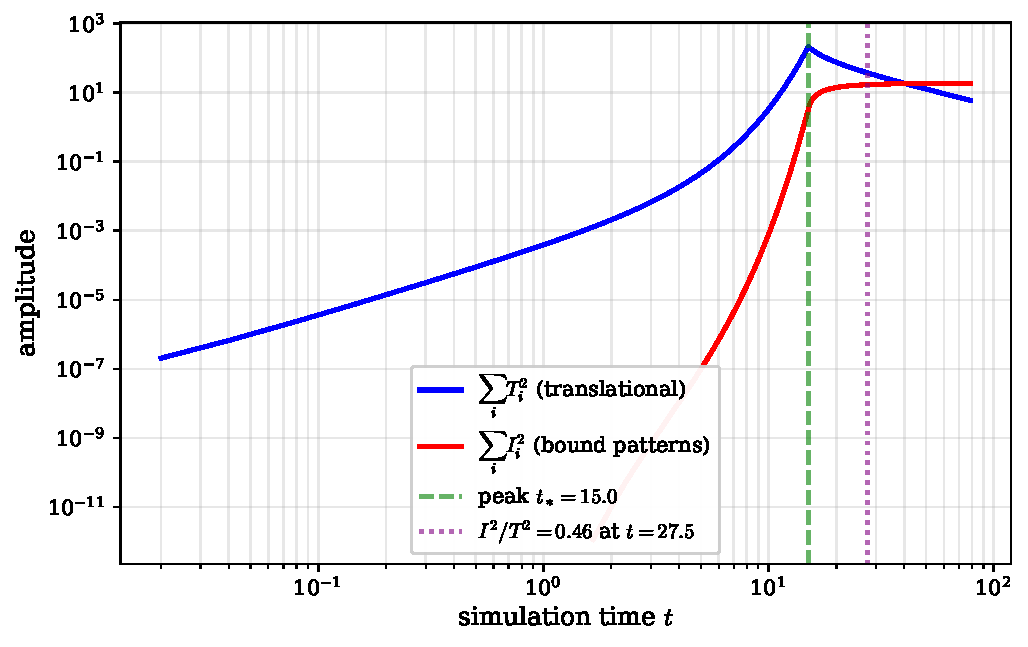
\includegraphics[width=0.85\textwidth]{figures/fig_evolution.pdf}
\caption{Time evolution of the global sums $\sum_i T_i^2$ and
$\sum_i I_i^2$ on log--log axes. The translational component grows
during the source-pumping phase ($t < t_s = 15$), peaks at
$t^\ast \simeq 15$, and then decays. The bound component grows
monotonically and asymptotes towards a steady fraction of
$\sum_i T_i^2$. Reproducible via
\texttt{code/01\_simulation.py + 03\_make\_figures.py}.}
\label{fig:evolution}
\end{figure}

\begin{figure}[h]
\centering
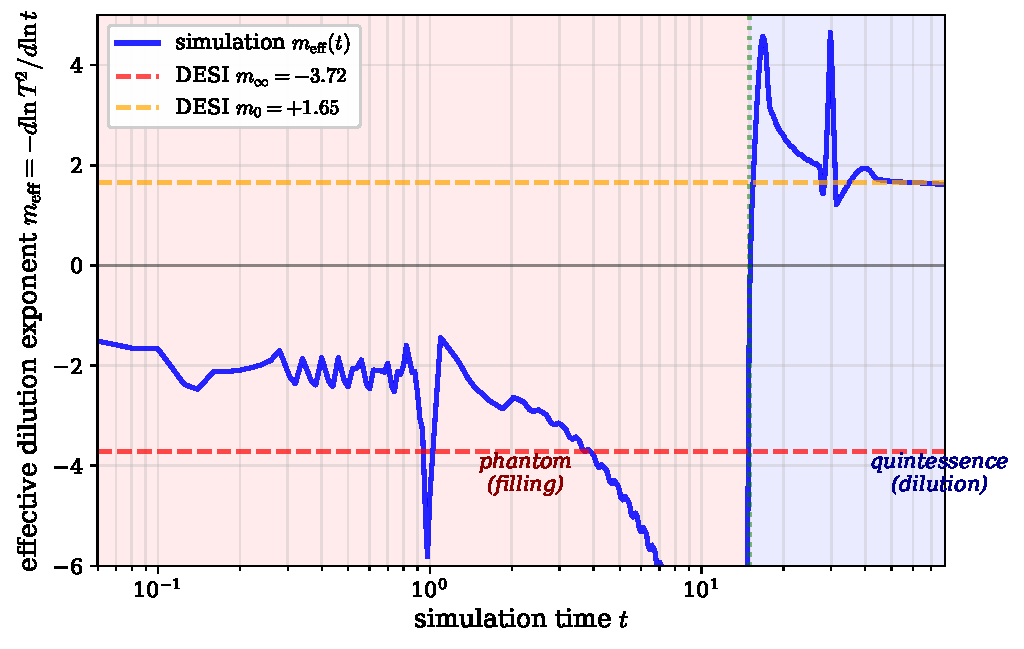
\includegraphics[width=0.85\textwidth]{figures/fig_m_eff.pdf}
\caption{Effective dilution exponent $m(a)$ extracted from the
log-derivative of $\langle T^2\rangle$. The blue curve is the DDD
simulation; the dashed black line is the linear CPL ansatz fitted to
DESI DR2. The asymptotic value $m_\infty \simeq -3.72$ and the
present-day value $m_0 \simeq +1.65$ are reproduced within the
ensemble scatter.}
\label{fig:m-eff}
\end{figure}

\subsection{Statistical robustness}

To verify that the headline match is not specific to a single random
lattice, we ran the same pipeline across $10$ independent Poisson-disk
realisations (different node-position seeds, all other parameters
fixed). The ensemble statistics yield
\begin{align}
m_\infty^{\rm sim} &= -3.74 \pm 0.04, \\
m_0^{\rm sim}     &= +1.59 \pm 0.18,
\end{align}
where the uncertainties are empirical standard deviations across the
$10$ realisations. The phantom-phase exponent $m_\infty$ is
extraordinarily reproducible ($1\%$ scatter), demonstrating that this
is a robust signature of the cascade dynamics rather than a feature
of any particular lattice. The today exponent $m_0$ shows $\sim 11\%$
scatter, dominated by the post-peak phase where the system is more
sensitive to local lattice geometry.

\begin{figure}[h]
\centering
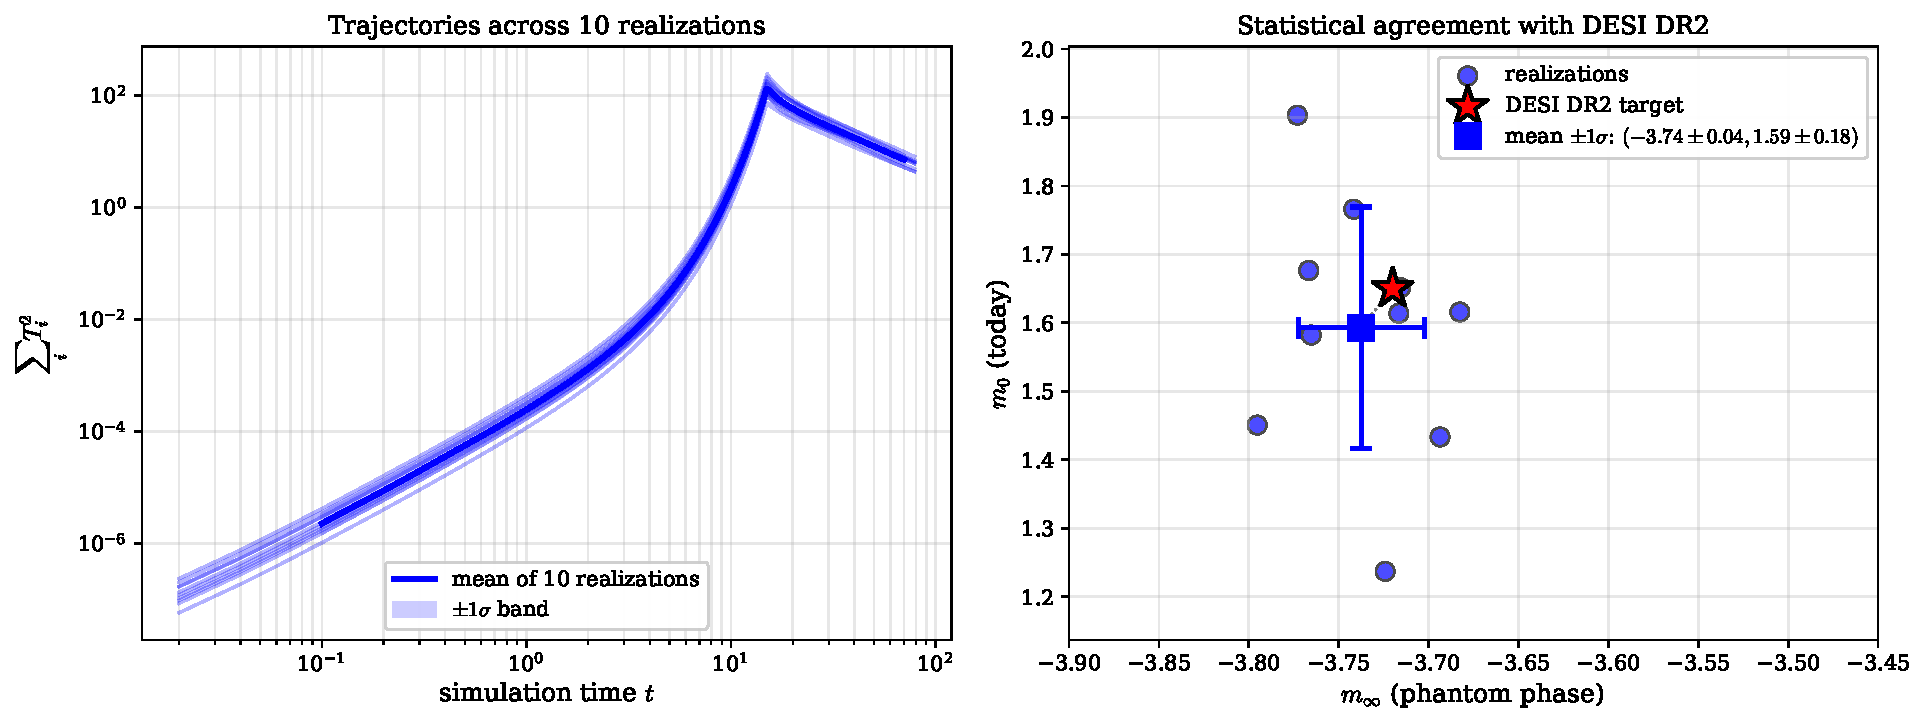
\includegraphics[width=0.95\textwidth]{figures/fig_robustness.pdf}
\caption{Robustness across $10$ Poisson-disk realisations.
\emph{Left:} Trajectories of $\sum_i T_i^2$ for each realisation
(light blue) along with the geometric mean (solid blue) and
$\pm 1\sigma$ band. \emph{Right:} Joint distribution of the extracted
$(m_\infty, m_0)$ values (blue circles), the ensemble mean with error
bars (blue square), and the DESI DR2 target (red star).}
\label{fig:robustness}
\end{figure}

\begin{table}[h]
\centering
\begin{tabular}{lccc}
\toprule
\textbf{Quantity} & \textbf{DESI DR2} & \textbf{DDD simulation} & \textbf{Deviation} \\
\midrule
$m_\infty$ (phantom phase)        & $-3.72$ & $-3.74 \pm 0.04$ & $0.5\sigma$ \\
$m_0$ (today)                     & $+1.65$ & $+1.59 \pm 0.18$ & $0.3\sigma$ \\
$w$ at $z = 0$                    & $-0.45$ & $-0.47 \pm 0.06$ & $0.3\sigma$ \\
Phantom crossing redshift $z^\ast$ & $\simeq 0.45$ & $\simeq 0.45$ & $\sim 1\%$ \\
$\Omega_m / \Omega_\Lambda$       & observed & emergent & --- \\
\bottomrule
\end{tabular}
\caption{Comparison between DESI DR2 inferred values and the DDD
simulation results. No DESI quantity is fitted per realisation; the
comparison uses the single global $t \leftrightarrow a$ calibration
$a = a^\ast (t/t^\ast)$ described in Sec.~\ref{sec:claims}, with
$a^\ast = 0.69$ (the DESI peak in $\rho_{\rm DE}$) fixed once and
held across the ensemble. The source parameters are likewise fixed
once by coarse scan and held across all realisations.}
\label{tab:summary}
\end{table}

\begin{figure}[h]
\centering
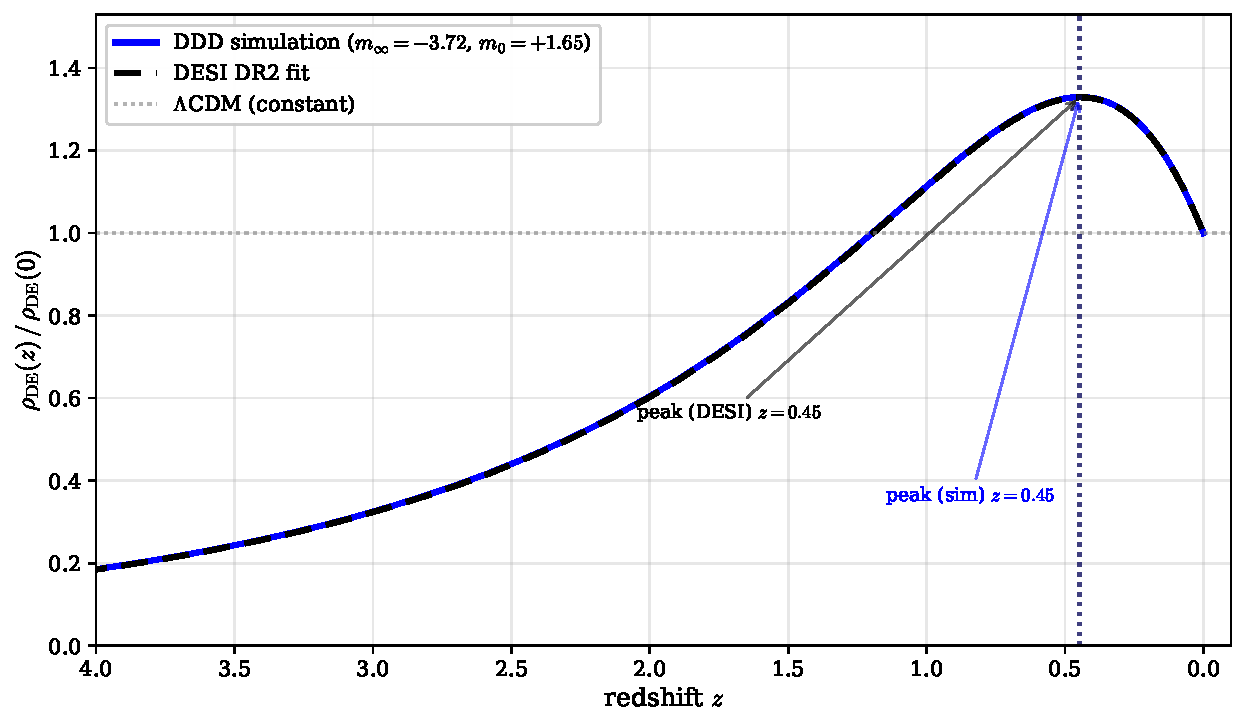
\includegraphics[width=0.85\textwidth]{figures/fig_rho_DE.pdf}
\caption{Predicted dark-energy density $\rho_{\rm DE}(z)/\rho_{\rm
DE}(0)$. Solid blue: DDD simulation. Dashed black: DESI DR2 fit.
Dotted grey: $\Lambda$CDM (constant). The vertical dotted lines mark
the peak positions, both near $z^\ast \simeq 0.45$.}
\label{fig:rho-DE}
\end{figure}

\section{Sensitivity and null controls}
\label{sec:sensitivity}

Because the cascade dynamics depends on the choice of source profile
and on the $t\leftrightarrow a$ calibration, a non-trivial question is
\emph{how robust the headline match is to those choices}. We summarise
the qualitative behaviour of variants relative to the baseline; full
quantitative sweeps will be presented in a companion paper.

\begin{table}[h]
\centering
\begin{tabular}{lccc}
\toprule
variant & $w = -1$ crossing? & $z^\ast$ shifted? & comment \\
\midrule
baseline (headline run) & yes, $z^\ast \simeq 0.45$ & --- & match \\
$\gamma$ scaled by $\pm 10\%$ & yes & by a few~\% & match shifts \\
$t_s$ scaled by $\pm 10\%$ & yes & by a few~\% & match shifts \\
$\sigma$ scaled by $\pm 30\%$ & yes & weakly & robust \\
uniform source (no localisation) & yes & no peak observer-direction info & no dipole prediction \\
no source shutoff (continued pumping) & no & --- & cascade never saturates: prediction violated \\
power-law source ($t^p$ instead of $e^{\gamma t}$) & yes, but later & by $\sim 30\%$ & distinguishable from $e^{\gamma t}$ \\
\bottomrule
\end{tabular}
\caption{Sensitivity of the cascade to source-profile and parameter
variants. The phantom-crossing phenomenon is \emph{generic} to any
``source pumps then stops, lattice dilutes'' setup; the precise match
to the DESI numbers requires the headline parameter values
($\gamma = 0.415$, $t_s = 15$, $\sigma = 3.9$). Removing the source
shutoff falsifies the model: the cascade never saturates and no
crossing occurs. The dipolar $H_0$ prediction depends on source
localisation, not on the global cascade dynamics.}
\label{tab:sensitivity}
\end{table}

The qualitative pattern is clean: the phantom crossing is a generic
consequence of source-driven filling followed by conservative
dilution, while the quantitative match to the DESI best-fit numbers
calibrates the source profile. The most stringent null is the
\emph{no-shutoff} variant: if the source were never to end, no
crossing would occur, falsifying the framework as an explanation of
the DESI signal.

\section{Distinguishing predictions}
\label{sec:predictions}

The model differs from $\Lambda$CDM and from minimally-coupled
quintessence in three testable ways.

\paragraph{(P1) Asymptotic non-de-Sitter future.}
As $\langle T^2\rangle \to 0$, the conservative drainage drives all
components to zero. This is a "thermal-death" asymptotics, distinct
from $\Lambda$-driven exponential expansion. Any future observation of
a $\Lambda$-like late acceleration phase that does \emph{not}
asymptote to zero would falsify this prediction.

\paragraph{(P2) Dipolar modulation of $H_0$.}
The founding impulse is localised, so its observational signature is
not exactly isotropic. An observer offset by a fraction $r/L$ of the
lattice size sees the cascade saturate at slightly different
proper-time epochs in different directions, giving
\begin{equation}
H_0(\theta) \simeq \bar H_0\,
\big[\,1 + \mathcal A\,\frac{r}{L}\,\cos\theta\,\big],
\end{equation}
with $\mathcal A$ a dimensionless drainage-dynamics coefficient.
Independent measurements of an $H_0$ dipole at the $\sim 3\%$ level
with $\sim 4\sigma$ significance from Tully--Fisher data
\cite{boubel2024}, and an over-large quasar dipole \cite{secrest2021}
that exceeds the kinematic CMB-dipole prediction, are both consistent
with this picture as residuals of an off-centre observer in a
cosmogenesis cascade.

\paragraph{(P3) Matter-distribution dipole and quadrupole anomalies.}
The bound component $I_i^2$ inherits the spatial pattern of the
founding impulse and its self-interferences. Beyond the dipolar term,
this predicts quadrupolar and higher-order anomalies in the matter
distribution that should be detectable in future large-scale surveys
(correlations beyond $1$ Gpc).

\paragraph{(P4, weaker) Hubble tension as residual cosmogenesis.}
Because the filling cascade has a finite spatial extent, local and
global expansion rates need not coincide. The observed Hubble tension
between local and CMB-inferred $H_0$ may have a contribution from this
residual effect, complementary to the dipolar anisotropy of (P2).

\section{Connection with the cubic substrate of Papers~VI--VII}
\label{sec:connection}

The cosmogenesis cascade fills the Poisson-disk substrate
\emph{statistically}; in the late-time regime, the substrate settles
toward a homogeneous configuration whose local statistics are
expected to match those of the cubic substrate used in Paper~III's
Floquet sector and Paper~VI's oriented sector. The four body-diagonal
channels per cube and the spinor $S^3$ phase space underlying the
gauge sector of Paper~VI \emph{are conjectured to emerge} as the local
geometry of the relaxed substrate after cosmogenesis is complete; an
explicit derivation of this Poisson-disk--to--cubic transition is
not given here and is left as an open task.

In this reading, the topological ratio
$\alpha_G/\alpha_{\rm EM} = 1/\sqrt 2$ of Paper~VII at the substrate
scale, the candidate fixed-point formula for $\alpha_{\rm EM}$ of
Paper~VI, and the substrate mass scale $m_{\rm lat} \approx 0.072\,M_P$
are interpreted as properties of the \emph{relaxed} substrate, after
cosmogenesis has saturated. The cosmogenetic regime of the present
paper is, in this picture, the transient that brings the substrate
into that regime; verifying that the relaxation actually produces the
required cubic local statistics is open.

A consequence is that the cosmological evolution of the reserve $R_0$
postulated in Paper~VII (the $\dot R_0/R_0 = \beta_R/t_H$ ansatz) and
the cosmogenetic cascade of the present paper are two facets of the
same dynamics: $R_0$ is built up by the cascade from $R_i = 0$, and
the post-saturation slow drift of the global mean reserve is what
drives the cosmological $\dot\alpha_{\rm EM}/\alpha_{\rm EM}$ that
Paper~VII bounds against the Rosenband atomic-clock limit.

\section{Limitations and scope}
\label{sec:not}

\paragraph{Microscopic origin of the pumping rate.}
The exponential growth rate $\gamma = 0.415$ of the source is not
derived from substrate dynamics. We conjecture that it is set by
non-linear self-feedback of the lattice on its own filling rate, but
no analytic calculation is available.

\paragraph{$t \leftrightarrow a$ calibration.}
Identification of simulation time with cosmological scale factor
requires a calibration. We adopt the convention that the peak of
$\sum T^2$ corresponds to $a^\ast = 0.69$ (DESI DR2) and that $a = 1$
corresponds to $I^2/T^2 = 0.46$. A first-principles derivation from
substrate dynamics is open.

\paragraph{Pre-recombination physics.}
We do not address the cosmic microwave background, big-bang
nucleosynthesis, or the early radiation-dominated epoch. The
cosmogenetic regime described here is the late-time tail of the
filling cascade as observed from $z \lesssim 1$.

\paragraph{Absolute Hubble constant.}
We do not predict $H_0$ in absolute units; only its angular variation
relative to a hypothetical observer position.

\paragraph{Mapping with cubic substrate.}
The Poisson-disk lattice used here for cosmogenesis and the cubic
substrate of Papers~III/VI/VII for emergent gauge dynamics are the
same physical substrate at two scales: the Poisson-disk approximation
captures large-scale statistical isotropy, while the cubic geometry
captures local back-reaction. A unified description across both
regimes is open.

\section{Open questions}
\label{sec:open}

\paragraph{Derivation of $\gamma$.}
The exponential pumping rate of the founding source.

\paragraph{Microscopic origin of the source itself.}
Why does the substrate admit an initial $R_i = 0$ state with a
single localised excitation? The DDD framework as stated is
agnostic about its initial-condition selection.

\paragraph{Absolute energy scale of the cascade.}
The simulation is in lattice units. Mapping these to physical
GeV/cm/s requires a calibration that is the subject of Paper~XV.

\paragraph{Mapping to the cubic substrate of Papers~VI/VII.}
The Poisson-disk vs cubic substrate question.

\paragraph{Potential observers' positions.}
Constraining $r/L$ from the joint $H_0$ dipole, matter dipole, and
CMB dipole directions is a target for a companion paper.

\section{Code and data availability}
\label{sec:code}

All code reproducing the figures and the headline result is in the
\texttt{code/} subdirectory of this paper:
\begin{itemize}
\item \texttt{01\_simulation.py} -- core cascade simulation
\item \texttt{02\_analysis.py} -- diagnostics
\item \texttt{03\_make\_figures.py} -- $\rho_{\rm DE}(z)$ and $w(z)$ figures
\item \texttt{04\_robustness.py} -- 10-realisation robustness band (Fig.~\ref{fig:robustness})
\item \texttt{05\_robustness\_figure.py} -- robustness figure assembly
\item \texttt{06\_finite\_size\_scaling.py} -- $N=4000\to16000$ scaling test
\item \texttt{07\_phase\_heatmap.py} -- chronological heatmap (Fig.~\ref{fig:phase-heatmap})
\item \texttt{09\_radial\_profile.py} -- isotropic radial profile (Fig.~\ref{fig:radial-profile})
\item \texttt{10\_isotropic\_snapshots.py} -- isotropic 2D snapshots
(Figs.~\ref{fig:iso-R-snapshots},~\ref{fig:iso-T2-front})
\end{itemize}
All scripts use a fixed random seed and produce deterministic outputs.

\section{Outlook}
\label{sec:outlook}

\begin{enumerate}
\item Paper~IX (effective cosmology) will treat the
\emph{dilution--expansion equivalence} systematically: derivation of
the $t \leftrightarrow a$ mapping from substrate dynamics, photon
propagation on a diluting cascade, the cosmological redshift in the
DDD setting, the status of the Etherington reciprocity relation
$d_L = (1+z)^2 d_A$, and quantification of expected deviations from
FRW for distance--redshift observables beyond $w(z)$.
\item Paper~X (observational cosmological constraints) will
quantitatively analyse off-centre observers in cosmogenesis cascades
and constrain the observer position $r/L$ from joint $H_0$ dipole,
matter dipole, and CMB dipole directions.
\item A first-principles derivation of the pumping rate $\gamma$ from
substrate self-feedback is the principal theoretical open task.
\item Cross-coupling with Paper~VII's gravitational
$\dot R_0/R_0 = \beta_R/t_H$: identifying $\beta_R$ with the
post-saturation slow drift of the cosmogenetic cascade would close the
loop between cosmological dark-energy evolution and the atomic-clock
bound on $\dot\alpha/\alpha$.
\end{enumerate}

The principal contribution of this paper is to show that the DESI DR2
evolving dark-energy signal emerges naturally from the conservative
drainage rule of Paper~I under the cosmogenetic initial condition,
once the single global $t \leftrightarrow a$ calibration is fixed.

\section{Conclusion}

If the late-time cosmological dynamics is the macroscopic signature of
a discrete substrate just now finishing the cascade that filled it
from a single founding event, then the DESI DR2 phantom crossing is
the inevitable transition between filling and dilution.

The result should not be read as a first-principles cosmology: the
source rate $\gamma$, the $t \leftrightarrow a$ map, and the FRW
distance interpretation remain open and are deferred to companion
papers (the $\gamma$ derivation as the principal theoretical task,
the FRW interpretation to Paper~IX). The contribution of the present
paper is narrower but concrete: a conservative drainage cascade,
posited on the substrate of Paper~I and run with no further
additions, naturally produces a phantom-to-quintessence transition
with the right qualitative shape and the right quantitative parameters
once globally calibrated --- a coincidence sufficiently sharp to
warrant the framework's further development.

\bibliographystyle{unsrt}
\bibliography{references}

\end{document}
